% =========================================================================
% fig_hd1_jsauri_desacoplamiento_345_138.tex
% Kirchhoff decoupling at Julio Sauri substation (345/230/138 kV)
% Dossier: TPWRS-SENI-142-2026 — SENI-142 benchmark
% Data: SENI142_RAMAS_LINEAS_Y_TRANSFORMADORES.csv + ARTEFACTO_B1 (sealed)
% =========================================================================
\documentclass[tikz,border=12pt]{standalone}
\usepackage[T1]{fontenc}
\usepackage[utf8]{inputenc}
\usepackage{amsmath}
\usetikzlibrary{arrows.meta,positioning,calc,backgrounds,fit}
\definecolor{seniNavy}{RGB}{26,54,93}
\definecolor{seniRed}{RGB}{155,44,44}
\definecolor{seniBlue}{RGB}{43,108,176}
\definecolor{seniGold}{RGB}{190,140,40}
\definecolor{seniGreen}{RGB}{39,103,73}
\tikzset{>={Stealth[length=2.5mm,width=1.8mm]},
         lbl/.style={font=\footnotesize,align=left},
         lblS/.style={font=\scriptsize,align=left}}
\begin{document}
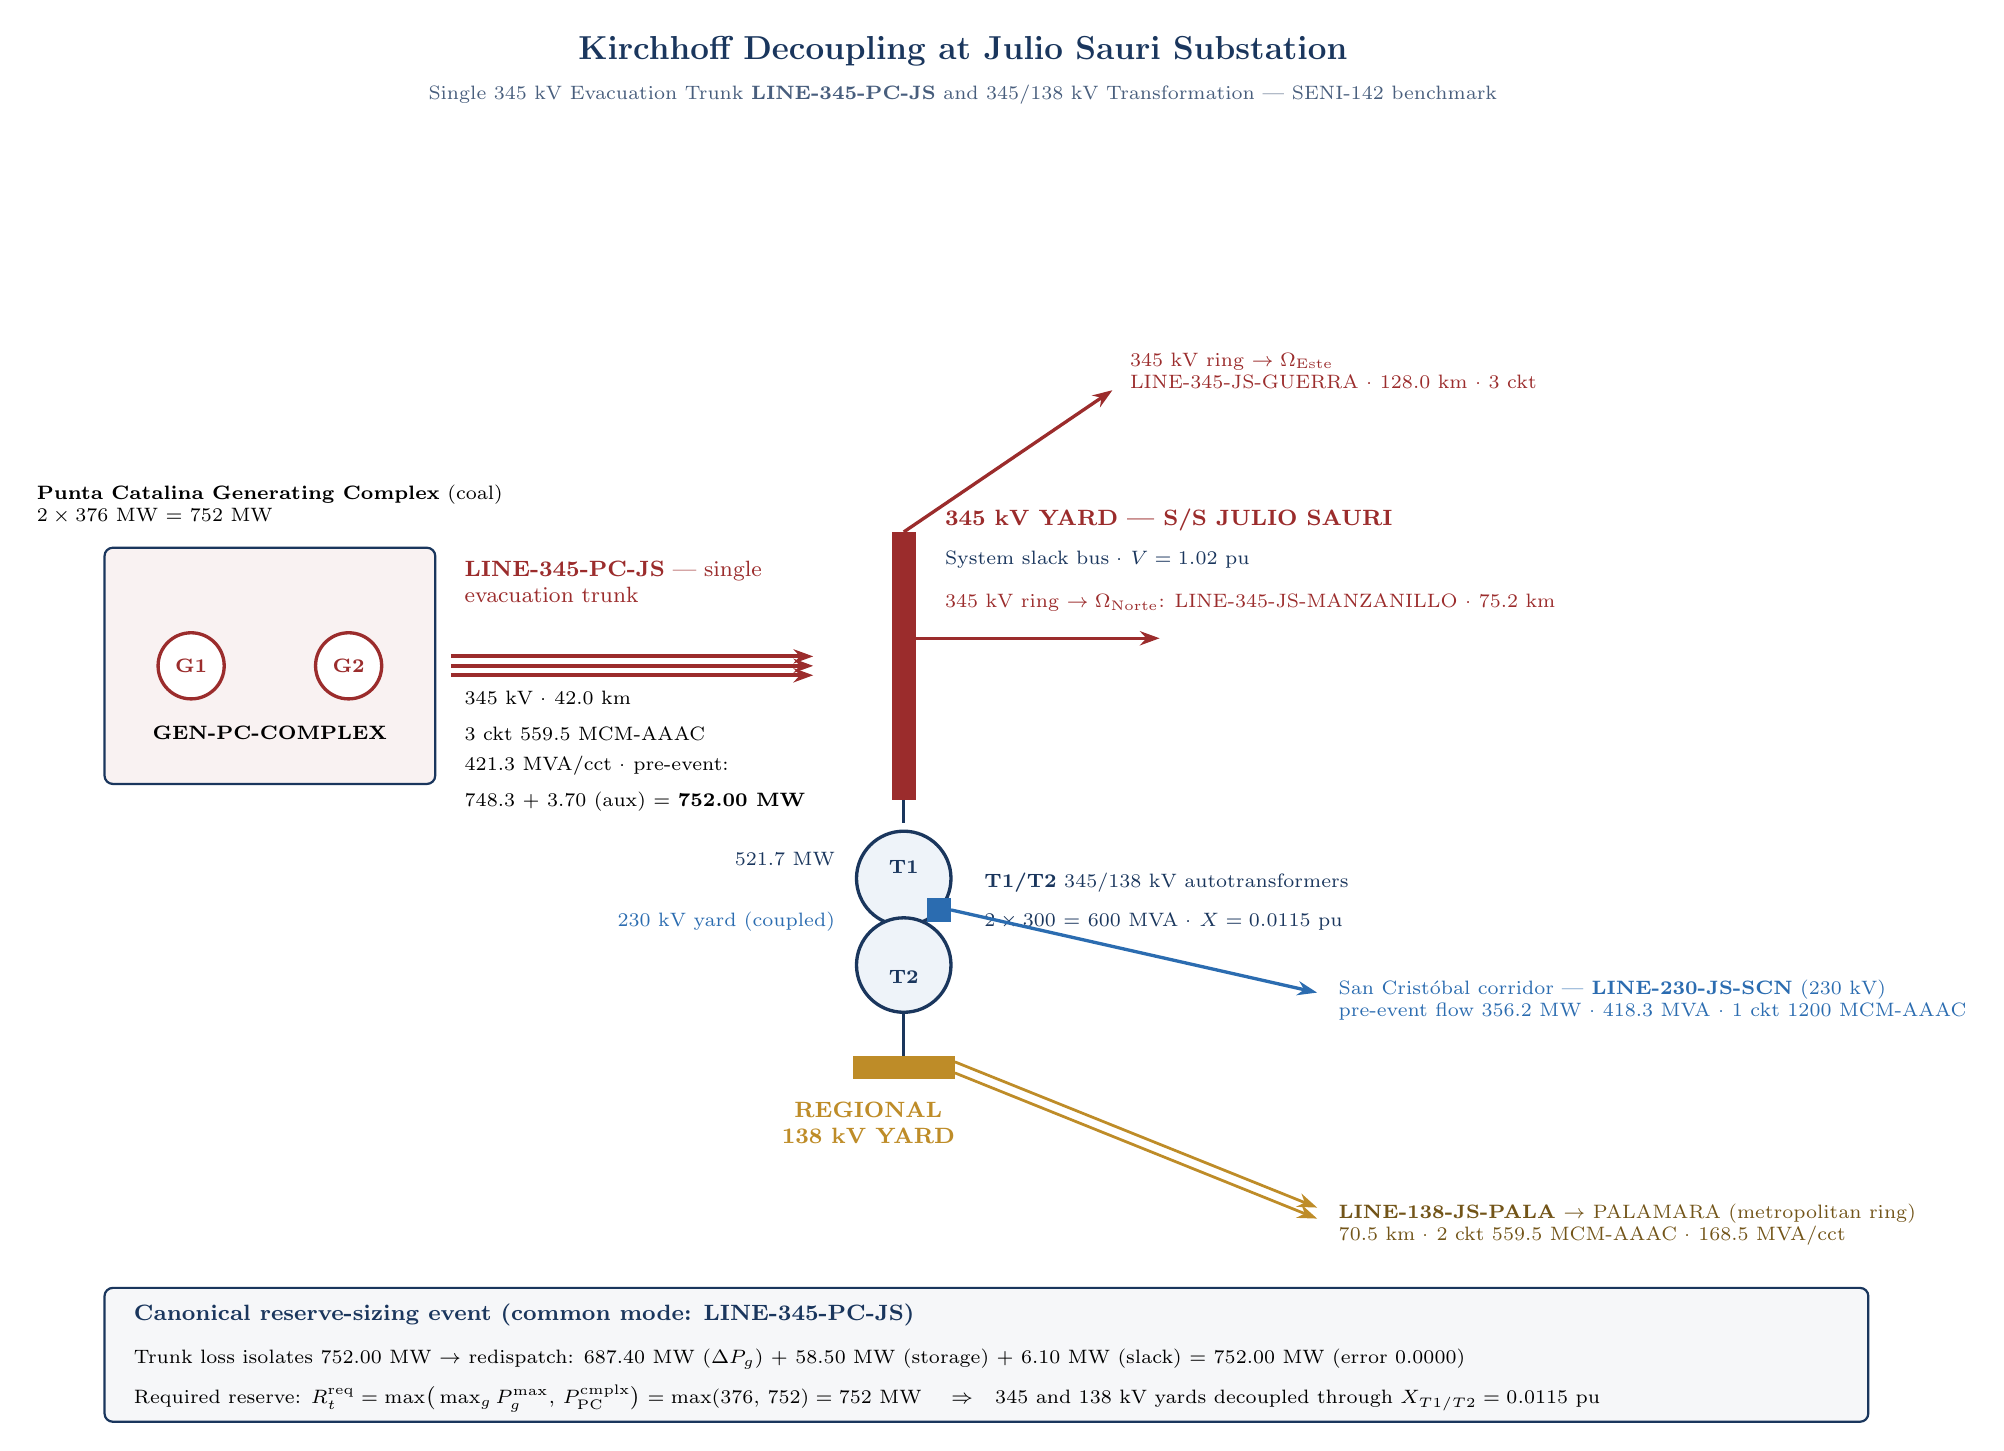
\begin{tikzpicture}[x=1cm,y=1cm]

% ------------------------------------------------------------ title
\node[lbl,font=\large\bfseries,seniNavy] at (8.8,7.8)
  {Kirchhoff Decoupling at Julio Sauri Substation};
\node[lblS,seniNavy!80] at (8.8,7.25)
  {Single 345 kV Evacuation Trunk \textbf{LINE-345-PC-JS} and 345/138 kV Transformation — SENI-142 benchmark};

% ------------------------------------------------- Punta Catalina complex
\draw[seniNavy,thick,rounded corners=3pt,fill=seniRed!6] (-2.1,-1.5) rectangle (2.1,1.5);
\draw[seniRed,very thick,fill=white] (-1.0,0) circle (0.42);
\draw[seniRed,very thick,fill=white] (1.0,0) circle (0.42);
\node[font=\scriptsize\bfseries,seniRed] at (-1.0,0) {G1};
\node[font=\scriptsize\bfseries,seniRed] at (1.0,0) {G2};
\node[lbl,font=\scriptsize] at (0,-0.85) {\textbf{GEN-PC-COMPLEX}};
\node[lbl,font=\scriptsize] at (0,2.05)
  {\textbf{Punta Catalina Generating Complex} (coal)\\ $2\times376$~MW~=~752~MW};

% ------------------------------------------------------- 345 kV trunk
\foreach \dy in {-0.12,0,0.12}{
  \draw[->,seniRed,line width=1.5pt] (2.3,\dy) -- (6.9,\dy);}
\node[lbl,seniRed,anchor=south west] at (2.35,0.68)
  {\textbf{LINE-345-PC-JS} — single\\ evacuation trunk};
\node[lblS,anchor=south west] at (2.35,-0.62)
  {345 kV · 42.0~km};
\node[lblS,anchor=south west] at (2.35,-1.07)
  {3 ckt 559.5~MCM-AAAC};
\node[lblS,anchor=south west] at (2.35,-1.52)
  {421.3~MVA/cct · pre-event:};
\node[lblS,anchor=south west] at (2.35,-1.97)
  {748.3 + 3.70 (aux)~=~\textbf{752.00~MW}};

% --------------------------------------------------------- 345 kV yard
\fill[seniRed] (7.9,-1.7) rectangle (8.2,1.7);
\node[lbl,anchor=west,font=\footnotesize\bfseries,seniRed] at (8.45,1.85)
  {345 kV YARD — S/S \textbf{JULIO SAURI}};
\node[lblS,anchor=west,seniNavy] at (8.45,1.35) {System slack bus · $V=1.02$~pu};

% 345 kV ring: upper-right exit (Guerra) and horizontal exit (Manzanillo)
\draw[->,seniRed,line width=1.2pt] (8.05,1.7) -- (10.7,3.5);
\node[lblS,seniRed,anchor=west] at (10.8,3.75)
  {345 kV ring $\to\Omega_{\text{Este}}$\\ LINE-345-JS-GUERRA · 128.0~km · 3 ckt};
\draw[->,seniRed,line width=1.2pt] (8.2,0.35) -- (11.3,0.35);
\node[lblS,seniRed,anchor=west] at (8.45,0.8)
  {345 kV ring $\to\Omega_{\text{Norte}}$: LINE-345-JS-MANZANILLO · 75.2~km};

% ------------------------------------------------- autotransformers T1/T2
\draw[seniNavy,line width=1.2pt] (8.05,-1.7) -- (8.05,-2.0);
\node[lblS,anchor=east,seniNavy] at (7.3,-2.45) {521.7~MW};
\draw[seniNavy,very thick,fill=seniBlue!8] (8.05,-2.7) circle (0.6);
\draw[seniNavy,very thick,fill=seniBlue!8] (8.05,-3.8) circle (0.6);
\node[font=\scriptsize\bfseries,seniNavy] at (8.05,-2.55) {T1};
\node[font=\scriptsize\bfseries,seniNavy] at (8.05,-3.95) {T2};
\draw[seniNavy,line width=1.2pt] (8.05,-4.4) -- (8.05,-4.95);
\node[lblS,anchor=west,seniNavy] at (8.95,-2.75)
  {\textbf{T1/T2} 345/138 kV autotransformers};
\node[lblS,anchor=west,seniNavy] at (8.95,-3.25)
  {$2\times300$~=~600~MVA · $X=0.0115$~pu};
% 230 kV tap of the autotransformer bank
\fill[seniBlue] (8.35,-3.25) rectangle (8.65,-2.95);
\node[lblS,anchor=east,seniBlue] at (7.3,-3.25) {230 kV yard (coupled)};

% --------------------------------------------------------- 138 kV yard
\fill[seniGold] (7.4,-5.25) rectangle (8.7,-4.95);
\node[lbl,anchor=north,font=\footnotesize\bfseries,seniGold,align=center] at (7.6,-5.42)
  {REGIONAL\\ 138 kV YARD};

% exit toward San Cristobal Norte (230 kV corridor) from the tap
\draw[->,seniBlue,line width=1.2pt] (8.65,-3.1) -- (13.3,-4.15);
\node[lblS,seniBlue,anchor=west] at (13.45,-4.25)
  {San Crist\'obal corridor — \textbf{LINE-230-JS-SCN} (230 kV)\\
   pre-event flow 356.2~MW · 418.3~MVA · 1 ckt 1200~MCM-AAAC};

% exit toward Palamara (2 x 138 kV circuits)
\foreach \dy in {-0.07,0.07}{
  \draw[->,seniGold,line width=1.0pt] (8.7,-5.1+\dy) -- (13.3,-6.95+\dy);}
\node[lblS,seniGold!60!black,anchor=west] at (13.45,-7.1)
  {\textbf{LINE-138-JS-PALA} $\to$ PALAMARA (metropolitan ring)\\
   70.5~km · 2 ckt 559.5~MCM-AAAC · 168.5~MVA/cct};

% ---------------------------------------------------- canonical event box
\draw[seniNavy,thick,rounded corners=3pt,fill=seniNavy!4] (-2.1,-9.6) rectangle (20.3,-7.9);
\node[lbl,anchor=west,font=\footnotesize\bfseries,seniNavy] at (-1.85,-8.25)
  {Canonical reserve-sizing event (common mode: LINE-345-PC-JS)};
\node[lbl,anchor=west,font=\scriptsize] at (-1.85,-8.8)
  {Trunk loss isolates 752.00~MW $\to$ redispatch: 687.40~MW $(\Delta P_g)$ + 58.50~MW (storage) + 6.10~MW (slack)~=~752.00~MW (error 0.0000)};
\node[lbl,anchor=west,font=\scriptsize] at (-1.85,-9.3)
  {Required reserve: $R_t^{\mathrm{req}}=\max\!\big(\max_g P_g^{\max},\,P_{\mathrm{PC}}^{\mathrm{cmplx}}\big)=\max(376,\,752)=752$~MW \quad$\Rightarrow$\quad 345 and 138 kV yards decoupled through $X_{T1/T2}=0.0115$~pu};

\end{tikzpicture}
\end{document}
